\documentclass[output=paper
,modfonts
,nonflat]{langsci/langscibook} 
%\bibliography{mwe2017bib3.bib} 
%% add all extra packages you need to load to this file 
\usepackage{graphicx}
\usepackage{tabularx}
\usepackage{amsmath} 
\usepackage{multicol}
\usepackage{lipsum}
%%%%%%%%%%%%%%%%%%%%%%%%%%%%%%%%%%%%%%%%%%%%%%%%%%%%
%%%                                              %%%
%%%           Examples                           %%%
%%%                                              %%%
%%%%%%%%%%%%%%%%%%%%%%%%%%%%%%%%%%%%%%%%%%%%%%%%%%%%
% remove the percentage signs in the following lines
% if your book makes use of linguistic examples
\usepackage{langsci/styles/langsci-gb4e} 
\usepackage{langsci/styles/langsci-optional} 
\usepackage{langsci/styles/langsci-lgr}
\usepackage{langsci/styles/langsci-bidi}
\usepackage{morewrites} 
%% if you want the source line of examples to be in italics, uncomment the following line
% \def\exfont{\it}

%\usepackage{enumitem} %Conflict with enumerate
\usepackage{lipsum}
\usepackage{multirow}
\usepackage{graphicx}
\usepackage{epstopdf}
\usepackage{wrapfig}
\usepackage{caption}
\usepackage{subcaption}
\usepackage{url}
\usepackage{relsize}
\usepackage{paralist}
\usepackage{tabularx} 
%\newfontfamily\Parsifont[Script=Arabic]{langsci/fonts/ScheherazadeRegOT_Jazm.ttf} 
\usepackage{latexsym}
\usepackage{tikz-dependency}
\usepackage{textgreek}
\usepackage{color}
\usepackage{newfloat}
\usepackage{hhline}
\usepackage{xspace}
\usepackage{booktabs}
\usepackage{verbatim} 
\usepackage{algorithm}
\usepackage[noend]{algpseudocode}
\usepackage{sidecap}
\usepackage{kantlipsum}
\usepackage{verbatimbox} 
\usepackage[usestackEOL]{stackengine}
\usepackage{tikz}
\usetikzlibrary{shapes.arrows}
\usepackage{todonotes}
\usepackage{csquotes}
\usepackage{amsmath}
%\usepackage[british]{babel}
\usepackage{mathtools}  % better amsmath
\usepackage{dcolumn}
\newcolumntype{d}[0]{D{.}{.}{2}}
\usepackage{cjhebrew} % Hebrew
\usepackage[normalem]{ulem}
\usepackage{qtree}
\usepackage{rotating}
\usepackage[section]{placeins} 
\usepackage{soulutf8}  % \ul command for underlining
% \usepackage{langsci/styles/langsci-bidi}

\usepackage{booktabs} %Salehi et al.
\usepackage{makecell} %Bhatia


%%% hyphenation points for line breaks
%% Normally, automatic hyphenation in LaTeX is very good
%% If a word is mis-hyphenated, add it to this file
%%
%% add information to TeX file before \begin{document} with:
%% %% hyphenation points for line breaks
%% Normally, automatic hyphenation in LaTeX is very good
%% If a word is mis-hyphenated, add it to this file
%%
%% add information to TeX file before \begin{document} with:
%% %% hyphenation points for line breaks
%% Normally, automatic hyphenation in LaTeX is very good
%% If a word is mis-hyphenated, add it to this file
%%
%% add information to TeX file before \begin{document} with:
%% \include{localhyphenation}
\hyphenation{
affri-ca-te
affri-ca-tes
an-no-tated
com-ple-ments
com-po-si-tio-na-li-ty
non-com-po-si-tio-na-li-ty
Gon-zá-lez
out-side
Ri-chárd
se-man-tics
STREU-SLE
}
\hyphenation{
affri-ca-te
affri-ca-tes
an-no-tated
com-ple-ments
com-po-si-tio-na-li-ty
non-com-po-si-tio-na-li-ty
Gon-zá-lez
out-side
Ri-chárd
se-man-tics
STREU-SLE
}
\hyphenation{
affri-ca-te
affri-ca-tes
an-no-tated
com-ple-ments
com-po-si-tio-na-li-ty
non-com-po-si-tio-na-li-ty
Gon-zá-lez
out-side
Ri-chárd
se-man-tics
STREU-SLE
}
%%add all your local new commands to this file

\newcommand{\smiley}{:)}

\renewbibmacro*{index:name}[5]{%
  \usebibmacro{index:entry}{#1}
    {\iffieldundef{usera}{}{\thefield{usera}\actualoperator}\mkbibindexname{#2}{#3}{#4}{#5}}}

% \newcommand{\noop}[1]{}

%add all your local new commands to this file

\newcommand{\ie}{i.e., }

% \newcommand{\noop}[1]{}

\newcommand{\blex}[1]{\textit{#1}\xspace}

\newcommand{\ngram}[1][]{$n$-gram{#1}\xspace}

\newcommand{\mwetype}[1]{\texttt{#1}\xspace}
\newcommand{\strongish}{\mwetype{strong}}
\newcommand{\weak}{\mwetype{weak}}
%\newcommand{\hard}{\mwetype{hard}}
\newcommand{\hard}{\textit{hard}}
%\newcommand{\mixed}{\mwetype{mixed}}
\newcommand{\mixed}{\textit{mixed}}

\newcommand{\gap}{$*$\xspace}
\newcommand{\zp}{\phantom{0}}

\newcommand{\figureref}[1]{Figure~\ref{#1}\xspace}
\newcommand{\tableref}[1]{Table~\ref{#1}\xspace}
\newcommand{\sectionref}[1]{Section~\ref{#1}\xspace}


\DeclareFloatingEnvironment[fileext=lod]{diagram}
\newcommand{\nothing}[1]{}

\DeclareOldFontCommand{\bf}{\normalfont\bfseries}{\mathbf}
\DeclareOldFontCommand{\it}{\normalfont\bfseries}{\mathbf}
\DeclareOldFontCommand{\sc}{\normalfont\bfseries}{\mathbf}


% \newcommand{\noop}[1]{}


\newcommand{\class}[1]{\texttt{#1}\xspace}
\newcommand{\localex}[1]{\textit{#1}\xspace}
\newcommand{\gl}[1]{``{#1}''\xspace}

\newcommand{\x}{\phantom{0}}

% Style guide provides these...

\newcommand{\localtabref}[2][]{Table#1~\ref{#2}\xspace}
\newcommand{\secref}[2][]{Section#1~\ref{#2}\xspace}
\newcommand{\localfigref}[2][]{Figure#1~\ref{#2}\xspace}

\newcommand{\eqnref}[2][]{Equation#1~\ref{#2}\xspace}

\newcommand{\REDDY}{ENC\xspace}
\newcommand{\BANNARD}{EVPC\xspace}

\newcommand{\MWE}{\ensuremath{\mathit{mwe}}}
\newcommand{\component}{\ensuremath{\mathit{component}}}

\newcommand{\spadeaff}{\ensuremath{\spadesuit}\xspace}
\newcommand{\clubaff}{\ensuremath{\clubsuit}\xspace}
\newcommand{\heartaff}{\ensuremath{\heartsuit}\xspace}
\newcommand{\diamondaff}{\ensuremath{\diamondsuit}\xspace}


\newcommand{\CS}[1]{\ensuremath{\mathit{CS}_{\mathit{#1}}}\xspace}

\newcommand{\CSsource}{\CS{L1}}
\newcommand{\CStarg}{\CS{L2N}}
\newcommand{\CSsourcetarg}{\CS{L1+L2N}}
\newcommand{\CSsvr}{\CS{SVR(L1+L2)}}
\newcommand{\CSstring}{\CS{string}}
\newcommand{\CSall}{\CS{all}}
\newcommand{\CSstringDS}{\CS{string+L1}}

%add all your local new commands to this file

\newcommand{\main}[1]{\textbf{#1}}

%\newcommand{\dataset}[1]{\textsc{#1}\xspace}

%\newcommand{\dataset}[1]{\textsc{#1}}

\newcommand{\feat}[1]{{\textsc{#1}}}
\newcommand{\swfeat}[2]{\feat{#1$_{#2}$}}
\newcommand{\bgfeat}[3]{\feat{#1$_{#2}$#1$_{#3}$}}
\newcommand{\tgfeat}[4]{\feat{#1$_{#2}$#1$_{#3}$#1$_{#4}$}}

\newcommand{\best}[1]{\textbf{#1}}
\newcommand{\hd}[1]{\textbf{#1}}


\newcommand{\dev}{\textsc{dev}}
\newcommand{\devAQ}{\dev$_{AQ}$}
\newcommand{\devDD}{\dev$_{DD}$}

\newcommand{\full}{\textsc{full}}
\newcommand{\fullAQ}{\full$_{AQ}$}
\newcommand{\fullDD}{\full$_{DD}$}

\newcommand{\expl}[1]{\emph{#1}}
% \mwegloss{original}{literal}{translat}
\newcommand{\mwegloss}[3]{\expl{#1} (lit.\ \expl{#2}) `#3'}


\renewbibmacro*{index:name}[5]{%
  \usebibmacro{index:entry}{#1}
    {\iffieldundef{usera}{}{\thefield{usera}\actualoperator}\mkbibindexname{#2}{#3}{#4}{#5}}}

% \newcommand{\noop}[1]{}

\newcommand{\compresslist}{
\setlength{\itemsep}{1pt}
\setlength{\parskip}{0pt}
\setlength{\parsep}{0pt}
\setlength{\leftmargin}{10cm}
}

\newcommand{\revcr}[1]{\textcolor{black}{#1}} % Revised by Carlos Ramisch
\newcommand{\revms}[1]{\textcolor{black}{#1}}  % Revised by Manon Scholivet
\newcommand{\revsc}[1]{\textcolor{black}{#1}}     % Revised by Silvio Cordeiro


\newcommand{\mcomment}[2]{\noindent{{\scriptsize\sffamily(\marginpar{\sffamily #1}#2)}}}
\newcommand{\ncomment}[2]{\noindent{{\sffamily\marginpar{\sffamily #1}#2}}}

%\newcommand{\car}[1]{\mcomment{\tiny{CAR}}{\textcolor{green}{#1}}} %Carlos' comments
%\definechangesauthor[name={Carlos Ramisch}, color={Green}]{cr}
\newcommand{\as}[1]{\mcomment{\tiny{AS}}{\textcolor{blue}{#1}}} %Agata's comments
\newcommand{\cara}[1]{\mcomment{\tiny{CR}}{\textcolor{red}{#1}}} %Carlos' comment
\newcommand{\mc}[1]{\mcomment{\tiny{MC}}{\textcolor{orange}{#1}}} %Marie's comments
\newcommand{\vv}[1]{\mcomment{\tiny{VV}}{\textcolor{gray}{#1}}} %Veronika's comments
\newcommand{\src}[1]{\mcomment{\tiny{SRC}}{\textcolor{magenta}{#1}}} %Silvio's comments
\newcommand{\fs}[1]{\mcomment{\tiny{FS}}{\textcolor{brown}{#1}}} %Federico's comments
\newcommand{\ad}[1]{\mcomment{\tiny{AD}}{\textcolor{brown}{#1}}} %Antoine's comments
\newcommand{\fc}[1]{\mcomment{\tiny{FC}}{\textcolor[rgb]{.7,0,.2}{#1}}} %Fabienne's comments
\newcommand{\iva}[1]{\mcomment{\tiny{IS}}{\textcolor{yellow}{#1}}} %Iva's comments
\newcommand{\bqz}[1]{\mcomment{\tiny{BQZ}}{\textcolor{gray}{#1}}} %Behrang's comments
\newcommand{\vg}[1]{\mcomment{\tiny{VG}}{\textcolor{magenta}{#1}}} %Voula's comments
\newcommand{\kuad}[1]{\mcomment{\tiny{KA}}{\textcolor{green}{#1}}} %Kübra's comments
\newcommand{\eb}[1]{\mcomment{\tiny{EB}}{\textcolor[rgb]{.3,.7,.2}{#1}}} %Eduard's comments
\newcommand{\guer}[1]{\mcomment{\tiny{GE}}{\textcolor{Mahogany}{#1}}} %Gulsen's comments
\newcommand{\jm}[1]{\mcomment{\tiny{JM}}{\textcolor{blue}{#1}}} %Johanna's comments
\newcommand{\capa}[1]{\mcomment{\tiny{CP}}{\textcolor{red}{#1}}} %Carla's comments
\newcommand{\lvdp}[1]{\mcomment{\tiny{LVDP}}{\textcolor{Emerald}{#1}}} %Lonneke's comments
%\newcommand{\ls}[1]{\mcomment{\tiny{LG}}{\textcolor{BlueViolet}{#1}}} %Luke's comments
\newcommand{\mvg}[1]{\mcomment{\tiny{MVG}}{\textcolor{magenta}{#1}}} %Maarten's comments
\newcommand{\yhk}[1]{\mcomment{\tiny{YHK}}{\textcolor{pink}{#1}}} %Yaakov's comments
\newcommand{\jk}[1]{\mcomment{\tiny{JK}}{\textcolor{NavyBlue}{#1}}} %Jolanta's comments
\newcommand{\sk}[1]{\mcomment{\tiny{SK}}{\textcolor{Orchid}{#1}}} %Simon's comments
\newcommand{\chli}[1]{\mcomment{\tiny{CHLI}}{\textcolor{pink}{#1}}} %Chaya's comments
\newcommand{\vm}[1]{\mcomment{\tiny{VM}}{\textcolor{blue}{#1}}} %Verginica's comments


% \newcommand*{\bfrac}[2]{\genfrac{}{}{0pt}{}{#1}{#2}}
%\newcommand{\tx}[1]{\text{#1}}
% \newcommand{\rarrow}[1]{\xRightarrow{#1}}
\newcommand{\mt}[1]{\mathit{#1}}

% JW: For highlighting newly written or modified parts.
\newcommand{\new}[1]{\textcolor{RedOrange}{\marginpar{\scriptsize\sffamily NEW}#1}}
% \newcommand{\new}[1]{#1}
\newcommand{\old}[1]{#1}
% \newcommand{\old}[1]{\textcolor{DarkGreen}{#1}}


%%%%%%%%%%%
%% STYLES FOR EXAMPLES
%%%%%%%%%%
%\newcommand{\lex}[1]{\textbf{#1}}  %Lexicalized component
%\newcommand{\ile}[1]{\textsl{#1}} %In-line example
%\newcommand{\gl}[1]{(lit.~\textsl{#1})} %Gloss

%%%%%%%%%%%
%% old version
%\newcommand{\gl}[1]{`\textsl{#1}'} %Gloss
%\newcommand{\tra}[1]{`{#1}'}  %Translation
%\newcommand{\tra}[1]{$\Rightarrow$\textsc{#1}}  %Idiomatic translation
%\newcommand{\tra}[1]{`#1'}  %Idiomatic translation
%\newcommand{\exgl}[2]{\ile{#1}~\gl{#2}} %Example with a gloss
%\newcommand{\extr}[2]{\ile{#1}~\tra{#2}} %Example with a translation
%\newcommand{\gltr}[2]{\gl{#1}~\tra{#2}} %Gloss with a translation
%\newcommand{\gltr}[2]{\gl{#1} $\Rightarrow$ \tra{#2}} %Gloss with a translation
%\newcommand{\exgltr}[3]{\ile{#1}~\gl{#2}~\tra{#3}} %Example with a gloss and a translation
%\newcommand{\exgltr}[3]{\ile{#1}~\gl{#2} $\Rightarrow$ \tra{#3}} %Example with a gloss and a translation

%%%%%%%%%%%
%% new version
%%%%%%%%%%
%\newcommand{\ile}[1]{\textsl{#1}} %In-line example with no gloss or translation
%\ewcommand{\exlit}[2]{\ile{#1}~\gl{#2}} %Example with a gloss
%\newcommand{\extr}[2]{\ile{#1}~\tra{#2}} %Example with a translation

%\newcommand{\lit}[1]{`\textsl{#1}'} %Literal translation
%\newcommand{\idio}[1]{`#1'}  %Idiomatic translation
%\newcommand{\exlit}[2]{\ile{#1}~\lit{#2}} %Example with a literal translation
%\newcommand{\exidio}[2]{\ile{#1}~\tra{#2}} %Example with an idiomatic translation
%\newcommand{\litidio}[2]{\lit{#1}$ \Rightarrow $\idio{#2}} %Literal and idiomatic translation
%\newcommand{\exlitidio}[3]{%\ile{#1}~\lit{#2}$\Rightarrow$\idio{#3}} %Example with a literal and a and idiomatic translation
%%%%%%%%%%%

%%%%%%%%%%%
%% in-line examples for languages in Latin script
%%%%%%%%%%
\newcommand{\lex}[1]{\textbf{#1}}  %Lexicalized component
\newcommand{\ile}[1]{\textsl{#1}} %In-line example  
\newcommand{\lit}[1]{`#1'} %Literal translation
\newcommand{\idio}[1]{`#1'}  %Idiomatic translation
\newcommand{\exlit}[2]{\ile{#1}~\lit{#2}} %Example with a literal translation
\newcommand{\exidio}[2]{\ile{#1}~\idio{#2}} %Example with an idiomatic translation
\newcommand{\litidio}[2]{\lit{#1}$~\Rightarrow~$\idio{#2}} %Literal and idiomatic translation
\newcommand{\exlitidio}[3]{\ile{#1}~\lit{#2}~$\Rightarrow$~\idio{#3}} %Example with a literal and a and idiomatic translation

%%%%%%%%%%%
%% in-line examples for languages in non-Latin script
%%%%%%%%%%
%\newcommand{\nlile}[1]{#1} %In-line example  
\newcommand{\nlile}[1]{{#1}} %In-line example  
\newcommand{\nltli}[1]{#1} %Transliterated in-line example  

\newcommand{\nlextlilit}[3]{\nlile{#1}~(\nltli{#2})~\lit{#3}} %Example with a transliteration and a literal translation
\newcommand{\nltlilit}[2]{\nltli{#1}~\lit{#2}} %A transliteration and a literal translation

\newcommand{\nlextliidio}[3]{\nlile{#1}~(\nltli{#2})~\idio{#3}} %Example with a transliteration and an idiomatic translation
\newcommand{\nltliidio}[2]{\nltli{#1}~\idio{#2}} %Example with an idiomatic translation
 
\newcommand{\nltlilitidio}[3]{\nltli{#1}~\lit{#2}~$\Rightarrow~$\idio{#3}} %Transliteration with a literal and an idiomatic translation
\newcommand{\nlextlilitidio}[4]{\nlile{#1}~(\nltli{#2})~\lit{#3}~$\Rightarrow$~\idio{#4}} %Example with a transliteration, a literal and an idiomatic translation
%%%%%%%%%%%

%% for compact lists
\newenvironment{senum}{
\begin{enumerate}
  \setlength{\topsep}{0pt}
  \setlength{\itemsep}{1pt}
  \setlength{\parskip}{0pt}
  \setlength{\parsep}{0pt}
}{\end{enumerate}\vspace{-.3em}}
\newenvironment{sitem}{
\begin{itemize}
  \setlength{\topsep}{0pt}
  \setlength{\itemsep}{1pt}
  \setlength{\parskip}{0pt}
  \setlength{\parsep}{0pt}
}{\end{itemize}\vspace{-.3em}}

%%%%%%%%%%%%%%%%%%
\newfontfamily\Parsifont[Script=Arabic]{ScheherazadeRegOT_Jazm.ttf} 
%\newfontfamily\Parsifont[Script=Arabic]{langsci/fonts/ScheherazadeRegOT_Jazm.ttf} 
\newcommand{\PRL}[1]{\RL{\Parsifont #1}}

%
% Silvio's additions
%%%%%%%%%%%%%%%%%%%%
\newcommand{\mweset}[1]{\ensuremath{\text{\{#1\}}}}
\newcommand{\xsub}[2]{\ensuremath{\text{#1}_{\text{#2}}}}
\newcommand{\mweG}[0]{\xsub{MWE}{Gold}}
\newcommand{\mweSa}[0]{\xsub{MWE}{S1}}
\newcommand{\mweSb}[0]{\xsub{MWE}{S2}}
\newcommand{\mweSc}[0]{\xsub{MWE}{S3}}
\newcommand{\tokG}[0]{\xsub{Tok}{Gold}}
\newcommand{\tokSa}[0]{\xsub{Tok}{S1}}
\newcommand{\tokSb}[0]{\xsub{Tok}{S2}}
\newcommand{\tokSc}[0]{\xsub{Tok}{S3}}
\newcommand{\tpmax}[0]{\xsub{TP}{max}}
%%%%%%%%%%%%%%%%%%%%
% End of Silvio's additions
%%%%%%%%%%%%%%%%%%%%


%%%%%%%%%%%%%%%%%%%
% Added by Salehi et al.
%%%%%%%%%%%%%%%%%%%
\newcommand{\dataset}[1]{\textsc{#1}\xspace}

\DeclareMathOperator{\len}{len}
\DeclareMathOperator{\Sim}{sim}
\DeclareMathOperator{\Mean}{mean}
\DeclareMathOperator{\LCS}{LCS}
\DeclareMathOperator{\LEVone}{LEV1}
\DeclareMathOperator{\LEVtwo}{LEV2}
\DeclareMathOperator{\alignedSequence}{alignedSequence}
\newcommand{\dictcc}{{\texttt dict.cc}\xspace}
%%%%%%%%%%%%%%%%%%%
% End of additions by Salehi et al.
%%%%%%%%%%%%%%%%%%%


 
\newcommand{\termdef}[1]{\textsc{#1}} %Term definition: the first occurrence of a term
 
 %% BQ added the following to get rid of [bibtexkey] in references
%\makeatletter
%\renewcommand{\@BIBLABEL}{\@emptybiblabel}
%\newcommand{\@emptybiblabel}[1]{}
%\makeatother

%\graphicspath{ {./Images/} }


%\newcommand{\mcomment}[2]{{\scriptsize\sffamily(\marginpar{\sffamily #1}#2)}}
\newcommand{\sm}[1]{\mcomment{\tiny{SM}}{\textcolor{blue}{#1}}}
\newcommand{\car}[1]{\mcomment{\tiny{CR}}{\textcolor{green}{#1}}}
%\newcommand{\vv}[1]{\mcomment{\tiny{VV}}{\textcolor{magenta}{#1}}}
%\newcommand{\as}[1]{\mcomment{\tiny{AS}}{\textcolor{orange}{#1}}}

\newcommand{\citealtv}[1]{\citeauthor{#1} \citeyear*{#1} [this volume]}

\newcommand{\pb}[1]{\textcolor{red}{\raisebox{.2ex}{\tiny PB:~}#1}}
\newcommand{\vk}[1]{\textcolor{blue}{\raisebox{.2ex}{\tiny VK:~}#1}}
\newcommand{\out}[1]{\textcolor[rgb]{0.8,0.8,0.8}{\textbf{#1}}}
\def\footurl#1{\footnote{\url{#1}}}

\newcommand*\rot{\rotatebox{90}} 



\newcommand{\pb}[1]{\textcolor{red}{\raisebox{.2ex}{\tiny PB:~}#1}}
\newcommand{\vk}[1]{\textcolor{blue}{\raisebox{.2ex}{\tiny VK:~}#1}}
\newcommand{\out}[1]{\textcolor[rgb]{0.8,0.8,0.8}{\textbf{#1}}}

%\def\Tref#1{Table~\ref{#1}}
%\def\Fref#1{Figure~\ref{#1}}
%\def\Sref#1{Section~\ref{#1}}
\def\footurl#1{\footnote{\url{#1}}}


\title{Paraphrases of verbal multiword expressions: the case of Czech light verbs and idioms} 
\author{%
Petra Barančíková\affiliation{Charles University}\lastand
    Václava Kettnerová\affiliation{Charles University} 
}
% \chapterDOI{} %will be filled in at production

%\epigram{}

\abstract{
In this chapter, we deal with two types of Czech verbal MWEs: light verb 
constructions and verbal idiomatic constructions. Many verbal MWEs are 
characterized by~the possibility of being paraphrased by single words. We 
explore paraphrasability of Czech verbal MWEs by single verbs in a 
semiautomatic experiment using word embeddings. Further, we propose a 
lexicographic representation of the obtained paraphrases enriched with 
morphological, syntactic and semantic information. We demonstrate 
one of its practical application in a machine translation experiment.
}

\title{Paraphrases of verbal multiword expressions: the case of Czech light verbs and idioms}

%\date{}

\begin{document}
\maketitle

\section{Introduction}

Multiword expressions (MWEs) are widely acknowledged as a serious challenge for 
both foreign speakers and many NLP tasks \citep{Sag2002a}. 
From various MWEs, those that involve verbs are of great significance 
as verbs represent the syntactic center of a sentence. \citet{baldwin2010multiword}
distinguish the following four types of verbal MWEs:

\begin{itemize}
\item 
verb-particle constructions (also referred to as particle verbs, or phrasal 
verbs), e.g., \textit{catch up}, \textit{put on}, \textit{swallow down},
\item
prepositional verbs, e.g., \textit{come across}, \textit{refer to},
\item
light-verb constructions (also referred to as verb-complement pairs, or support 
verb constructions), e.g., \textit{do a report}, \textit{give a kiss}, 
\textit{make an attempt}, %\textit{take a bath}, \textit{have pity}, 
\item
verb-noun idiomatic constructions (also referred to as VP idioms), e.g., 
\textit{spill the beans}, \textit{pull strings}, \textit{shoot the breeze}.
\end{itemize}


In this chapter, we focus on two particular types of Czech verbal MWEs, namely
on~light-verb constructions (LVCs) and idiomatic verb constructions (IVCs) as 
they represent  MWEs also in Czech in contrast to the first two types that are 
primarily expressed as~single prefixed verbs. 

We explore the possibility of expressing these two types of MWEs by single 
synonymous verbs, which is considered to be one of their prototypical features, 
see e.g. \citet{chafe-68} and \citet{fillmore-88}. The motivation for this work 
lies in the fact that paraphrases greatly assist in a wide range of NLP 
applications, let us mention information retrieval \citep{wallisinformation}, 
machine translation \citep{Madnani:2013,Callison-Burch:2006,Marton:2009} 
or machine translation evaluation \citep{Kauchak:2006,Zhou:2006,BaRoImprovingEvaluation2014}. 

The content of this chapter is an extended version of \citet{barancikova2017paradi}.
In addition, it is enhanced with IVCs and linguistic properties of LVCs and IVCs 
that are relevant to the paraphrasing task are discussed in detail. The 
new version of the paraphrase dictionary is larger and it provides a more 
elaborated set of morphological, syntactic and semantic features, including 
information on aspects and aspectual counterparts of verbs.

This chapter is structured as follows. First, linguistic properties of LVCs and 
IVCs  are discussed (\sectref{liguistic}) and related work on their paraphrases is 
introduced. Second, a paraphrasing model is proposed, namely the 
selection of~LVCs and IVCs, an automatic extraction of candidates for their 
paraphrases and their manual evaluation are described in detail (\sectref{CPs}). 
Third, the resulting data and their representation in a dictionary of 
paraphrases are introduced (\sectref{results}). Finally, in order to present one 
of many practical applications of~this dictionary, a~random sample of 
paraphrases of LVCs is used in~a~machine translation experiment (\sectref{evaluation}). 
%The results of this experiment showed that substituting LVCs for their single word paraphrases improves quality of machine translation.

\section{Linguistic properties of LVCs and IVCs}
\label{liguistic}
Both LVCs and IVCs represent verbal multiword units: they are composed 
of~separate words that, however, refer to an extralinguistic reality as a whole. 
Their linguistic properties relevant for their paraphrasability by single verbs 
are introduced below. 

\subsection{Light-verb constructions}
\label{LVCs}
The theoretical research on light-verb constructions is characterized by 
an~enormous diversity in~terms and analyses used, see esp. \citet{amberber-10} 
and \citet{alsina-97}. Here, we use the term  LVC for a~multiword unit within 
which the verb -- not retaining its full semantic content -- provides rather 
grammatical functions and to which the main predicative content is contributed 
by a~noun; as a~result, such a multiword unit serves as~a~single predicative 
unit, see e.g. \citet{algeo-95}, \citet{alsina-97} and 
\citet{butt-2010}.\footnote{Besides predicative nouns, adjectives, adverbs and
verbs can also serve as predicative elements. These cases are left aside 
here.} In contrast to IVCs, predicative nouns in LVCs have the same meanings 
as in nominal structures, meanings of light verbs are rather impoverished when 
compared with their full verb counterparts, see \sectref{IVCs}. 

In the Czech language, the central type of LVCs are represented by LVCs in 
which predicative nouns are expressed as a direct or indirect object of a 
light verb (e.g., \exlitidio{dostat strach}{to get fear}{to get afraid}, 
\textit{vzdát úctu} `to pay tribute', and \exlitidio{vyvolat pobouření}{to provoke indignation}{to 
cause uproar}). 
The LVCs in which a predicative noun occupies an adverbial of the light verb, 
(e.g., \textit{dát do pořádku} `to put in~order', \textit{mít pod kontrolou} 
`to have under control', \exlitidio{mít na starosti}{to 
have on care}{to be responsible}) exhibit greater syntactic and morphological fixedness than the 
central type of LVCs \citep{radimsky-10}.

As~single predicative units, most LVCs have their single predicative 
counterparts by~which they can be paraphrased. A single verb paraphrase can be
either morphologically related, or non-related with the predicative noun 
representing the nominal component of the paraphrased LVC. For example, the~LVCs 
\textit{dát polibek} and \textit{dát pusu} `give a kiss' can be both paraphrased 
by the verb \textit{políbit} `to kiss', which is morphologically related only 
with the nominal component of  the first LVC. There is no synonymous verb 
morphologically related to the nominal component of the second LVC.

In~contrast to their single predicative paraphrases, LVCs manifest greater 
flexibility in their modification, compare e.g. adjectival modifiers of~the LVC 
\textit{dát polibek} `give a~kiss' and the corresponding adverbial modifiers 
of~its single verb paraphrase \textit{políbit} `to kiss':  
\textit{dát váš\-ni\-vý/něž\-ný/let\-mý/man\-žel\-ský/má\-jo\-vý/smr\-tí\-cí 
po\-li\-bek} `give a pas\-sion\-ate/ten\-der/fleet\-ing/mar\-riage/May/fa\-tal 
kiss' vs. \textit{váš\-ni\-vě/ něž\-ně/let\-mo/*man\-žel\-sky/*má\-jo\-vě/*smr\-tel\-ně 
po\-lí\-bit} `to kiss pas\-sion\-ate\-ly/ten\-der\-ly/fleet\-ing\-ly/*mar\-riage\-ly/*May\-ly/?fa\-tal\-ly'.  Easier modification of LVCs is often considered a motivation for their use \citep{brinton-99}.

Another motivation lies in the possibility to structure the expressed event 
in~a~more subtle way than single verbs allow. For example, in Czech various 
combinations of the grammatical aspect of light verbs and the number of 
predicative nouns allow for the expression of several meanings that cannot be 
expressed with single verbs; these cases require lexical modification, see 
\tabref{aspect}.

\begin{table}[tb]
	\centering
	\begin{tabular}{lccc}
	 \lsptoprule
	   \multirow{2}{*}{LVC} & Single verb & Lexical        & \multirow{2}{*}{Example} \\
	                     & paraphrase &  modification   &   \\ \midrule
		\multirow{4}{*}{sg \& pf}   & \multirow{4}{*}{pf} &  \multirow{4}{*}{no} &  \textit{Petr dal Janě polibek}. \\ 
		                            &                     &                      &  `Peter gave a~kiss to Jane.' \\
		                            &                     &                      &   $\thicksim$ \textit{Petr Janu políbil}. \\
		                            &                     &                      &   `Peter kissed Jane.'\\ \hline
 		\multirow{4}{*}{pl \& impf} & \multirow{4}{*}{impf} & \multirow{4}{*}{no}     &  \textit{Petr dával Janě polibky.} \\
 		                            &                       &                         & `Peter gave kisses to Jane.' \\ 
                                  &                       &                         & $\thicksim$ \textit{Petr Janu líbal}. \\
                                  &                       &                         & `Peter was kissing Jane.' \\ \hline  		                                                                                  
		\multirow{4}{*}{pl \& pf}  & \multirow{4}{*}{pf}  & \multirow{4}{*}{yes}    &    \textit{Petr dal Janě polibky}. \\
		                            &                       &                        &    `Peter gave several kisses to Jane.' \\ 
                                  &                       &                        &     $\thicksim$ \textit{Petr Janu několikrát políbil.} \\
                                  &                       &                        &     `Peter kissed Jane several times.' \\ \hline
		\multirow{4}{*}{sg \& impf} & \multirow{4}{*}{impf}   & \multirow{4}{*}{yes}  &   \textit{Petr Janě dával polibek.} \\
		                            &                       &                       &   `Peter was giving a kiss to Jane.' \\ 
		                            &                       &                       &   $\thicksim$ \textit{Petr Janu právě líbal.}  \\
		                            &                       &                       &    `Peter was just kissing Jane.'\\    
	\lspbottomrule       
	\end{tabular}
	\caption{Possible combinations of the grammatical aspect of the light verbs 
	\textit{dát}$^{pf}$, \textit{dávat}$^{pf}$ `to give' and the number of the 
	noun \textit{polibek} `kiss' and their paraphrasability by the perfective and 
	imperfective single verbs \textit{políbit}$^{pf}$ and \textit{líbat}$^{impf}$ 
	`to~kiss', respectively. Let us emphasize that the single verb paraphrases of 
	the last two combinations require to be lexically modified -- by the words 
	\textit{několikrát}  `several times' and \textit{právě} `just', respectively.}
	\label{aspect}
\end{table}

Finally, in many cases, the selection of~different light verbs allows for 
 perspectivization of the expressed event from the point of view of 
its different participants, see 
esp. \citet{depling-lvc-2015}. For example, beside the light verb \textit{dát} 
`to give', the noun \textit{polibek} `kiss' can select the light verb 
\textit{dostat} `to get' as well. The LVC \textit{dát polibek} `to give a kiss' 
promotes a kisser in the subject position while 
the LVC \textit{dostat polibek} `to get a kiss' puts a kissee into this position. Both these LVCs are paraphrasable by a single verb \textit{políbit} `to kiss', however, with different values of the 
grammatical voice: the LVC \textit{dát polibek} `to give a~kiss' 
can be paraphrased by the verb \textit{políbit} `to kiss' in the active voice  
(e.g., \textit{Petr dal Janě polibek.} `Peter gave a kiss to Jane.' $\thicksim$ 
\textit{Petr Janu políbil.} `Peter kissed Jane.') while the LVC \textit{dostat 
polibek} `to get a kiss' requires the passive voice of~the verb \textit{políbit} 
`to kiss' (e.g., \textit{Jana dostala od Petra polibek.} `Jane got a kiss from 
Peter.' $\thicksim$ \textit{Jana byla políbena od Petra.} `Jane was kissed by Peter'.)

%\noindent
%\smallskip
%\textbf{Remarks on Idiomatic light-verb constructions.}
%In Czech, the borderline between LVCs and verbal idioms is represented by LVCs 
%in which the predicative noun is expressed as an adverbial of the light verb, 
%e.g., \textit{dát do pořádku} `to put in~order', \textit{mít pod kontrolou} 
%`to have under control', \textit{mít na starosti} `to be responsible, lit. to 
%have on care' referred here to as idiomatic LVCs (ILVCs). ILVCs represent an 
%understudied language phenomenon, for Czech see e.g., \citet{radimsky-10}. 

%In comparison with LVCs with predicative nouns expressed as the direct or 
%indirect object, idiomatic LVCs are more fixed. First, they do not allow 
%for adjectival modifiers as easily as LVCs. For example, the noun \textit{úmysl} 
%`intention' in the idiomatic LVC  \textit{mít v úmyslu} `to intend, lit. to 
%have in intention' can be modified only by the adjective \textit{nejmenší} and 
%\textit{sebemenší} `slightest' only on condition that the light verb is 
%negated (\textit{Nemám v nejmenším úmyslu ti radit.} `I do not have the 
%slightest intention to advise you.'). Second, the number of the predicative noun 
%is typically limited either to the singular \textit{vzít v 
%úvahu$^{sg}$/*úvahy$^{pl}$} `to take into consideration', or to the plural 
%\textit{nechat na pochybách$^{pl}$/*pochybě$^{sg}$} `to leave in doubt, lit. 
%to leave on doubts'.

%Finally, a predicative noun in idiomatic LVCs usually selects a restricted set 
%of~light verbs; thus the possibilities to perspectivize of the expressed event 
%from the point of view of different participants are not varied with idiomatic 
%LVCs. For~example, the noun \textit{pořádek} `order' selects only the light verb 
%\textit{dát} `to give'; the resulting idiomatic LVC \textit{dát do pořádku} `to 
%put in order' perspectivizes the event from the point of `Agent'.
%Idiomatic LVCs represent an 
%understudied language phenomenon, for Czech see e.g., \citet{radimsky-10}.

\subparagraph{LVCs in NLP.} 
%The information on LVCs is a part of several lexical resources containing 
%manually annotated data. For instance, LVCs are represented in syntactically 
%rich annotated corpora from the family of the Prague Dependency Treebanks: the 
%Prague Dependency Treebank 3.0 (PDT)\footurl{http://ufal.mff.cuni.cz/pdt3.0} 
%andthe Prague Czech-English Dependency Treebank 
%2.0\footurl{http://ufal.mff.cuni.cz/pcedt2.0/en/index.html}, see 
%\citet{pdt-3-0-2013} and \citet{biblio:HaHaAnnouncingPrague2012}.
%Further, the PropBank\footurl{https://verbs.colorado.edu/~mpalmer/projects/ace.html} 
%project has been recently enhanced with the information on LVCs; the annotation 
%scheme of LVCs in~PropBank is thoroughly described in \citet{hwang:2010}. Finally, 
%the Hungarian corpus of LVCs based on~the~data from the Szeged Treebank has been 
%built \citep{Vincze:2010}.}
One of the trending topics concerning LVCs in the NLP community is their automatic 
identification. In~this task, various statistical measures often 
combined with information on syntactic and/or semantic properties of LVCs are
employed, see e.g., \citet{Bannard:2007} and \citet{fazly:2005}. The automatic 
detection benefits especially from parallel corpora representing valuable 
sources of data in which LVCs can be automatically recognized via word alignment, 
see e.g. \citet{Chen:2015}, \citet{Caseli2010}, \citet{Sinha:2009}, \citet{ZarrieB:2009}.     
%\newcite{Chen:2015} presents a supervised classifier of English light verb 
%constructions based on dependency parsing and external ontologies such as WordNet.
However, work on paraphrasing LVCs is still not extensive. For example, a 
paraphrasing model has been proposed within the Meaning$\leftrightarrow$Text 
Theory \citep{ZolkovskijMelcuk65}; its representation of LVCs by means of lexical 
functions and rules applied in the paraphrasing model are thoroughly described in \citet{ramos-07}. 
Further, \citet{Fujita:2004} presents a paraphrasing model which 
takes advantage of semantic representation of LVCs by lexical conceptual structures. 
As with our method proposed in \sectref{CPs}, their model also takes into 
account several morphological and syntactic features of LVCs, which have turned out 
to be highly relevant for the paraphrasing task.   

\subsection{Idiomatic Verbal Constructions}
\label{IVCs}
Despite their low frequency, IVCs form a substantial part of a lexis, see e.g. \citet{baldwin2010multiword}, \citet{Sag2002a}, \citet{cowie-01}.  Similarly to LVCs, 
definitions of~idioms vary depending on diverse purposes of their description, see e.g., \citet{healy-68}, \citet{fraser-70}, \citet{van1992incremental}, and \citet{nunberg-94}. 

Here, we define an IVC as a verbal multiword unit that exhibits strong lexical 
co-occurrence restrictions so that at least one of its parts cannot be used with 
the same meaning outside the given multiword unit. The idiomatic meaning of 
individual components of IVCs is reflected in the fact that they are only rarely 
interchangeable with words of similar meanings. 
IVCs thus represent highly conventionalized multiword units, see e.g. 
\citet{everaert-14}, \citet{granger-08}, \citet{cowie-01}. IVCs can 
exhibit the following specific properties, see e.g. \citet{burger-07}, 
\citet{cermak-01}, \citet{everaert-14}:

\begin{itemize}
\item
markedness at the syntactic and/or morphological level: e.g., \exlitidio{vzít za 
své}{take as one's own}{to be no more} (syntactically marked as the reflexive 
adjective \textit{své} does not modify any noun), and \exlitidio{nalít někomu 
čistého vína}{to pour someone pure wine}{to tell someone the honest truth} 
(morphologically marked due to the partitive genitive of the noun \textit{víno} 
`wine', which is highly restricted in the contemporary Czech),
 
\item
figuration: e.g., \textit{vstát z mrtvých}, `raise the dead' (as it involves 
metaphor), \textit{pověsit se někomu na krk} `to hang around someone's neck' 
(as it involves metonymy),

\item
fixedness at syntactic and/or morphological level: e.g., 
\textit{postavit někoho na nohy} `to put someone back on his feet' 
(syntactically fixed as it cannot be transformed into the passive structure), 
and \exlitidio{přijít na jiné myšlenky}{to
come to different ideas}{to find something else to think about} (morphologically fixed as the noun \textit{myšlenka} 
`idea' can have only the plural form),

\item
proverbiality: IVCs are typically used for recurrent socially significant 
situations, implying often their subjective evaluation (e.g., \textit{vidět 
někomu do duše} `to see right through someone'),

\item
informality: IVCs are typically of informal register (e.g., \exlitidio{strčit si 
něco za klobouk}{to put something behind a hat}{to stick it up one's jumper}).
\end{itemize}

Some IVCs can be paraphrased by a single word verb, see e.g., the IVC 
\textit{podat někomu pomocnou ruku} `to give someone helping hand' and its 
single verb paraphrase \textit{pomoci} `to help'. However, many IVCs are 
paraphrasable rather by a~whole syntactic structure, see e.g., the IVC 
\exlitidio{mít slovo}{to have a word}{to be someone's turn to speak}.

 \subparagraph*{IVCs in NLP.} There is considerable work focused on automatic 
identification of idioms in the text and their extraction
\citep{cook-07,li-2009,muzny2013,peng-15,Katz06automaticidentification}. 
However, little attention has been paid to paraphrases of idioms. Let us 
introduce two works focused on paraphrases of idioms. First, \citet{pershina-15} 
identifies synonymous idioms based on their dictionary definitions  and their 
occurrences in tweets. Similarly, \citet{liu2016phrasal} generates paraphrases 
of idioms using  dictionary entries. However, in Czech, there are no lexical
resources available for NLP applications providing information on idioms. 


\section{Paraphrase model}
\label{CPs}

%\emph{ParaDi} was built on~a~semi-automatic basis. First, candidates for single 
%verb paraphrases of selected CPs have been automatically identified in~large  
%monolingual data using \emph{word2vec}, a shallow neural network. The list of 
%these candidates has been then manually checked and further refined. In many  
%cases, if CPs are to be correctly paraphrased by the identified single 
%predicative verbs, these verbs require certain semantic and/or syntactic
%modifications.

In this section, the process of paraphrase extraction is described in detail. 
First, we present the selection of LVCs and IVCs (\sectref{sec:datasets}). For 
their paraphrasing, we had initially intended to use some of the existing 
resources, however, they turned out to be completely unsatisfactory for 
our task.

First, we used the \emph{ParaPhrase DataBase} (PPDB) \citep{ppdb}, 
the largest paraphrase database available for the Czech language. PPDB was 
created automatically from large parallel data. Unfortunately, there were only 
54 candidates for single verb paraphrases of LVCs present. A manual analysis of 
these candidates has shown that only 2 of them have been detected correctly, the 
rest was noise in PPDB. Similarly for idioms, PPDB contained a correct single 
verb paraphrase for only 6 IVCs from our data (i.e. about 1\%). As this number 
is clearly insufficient, we chose not to use parallel data for paraphrasing.

%\out{To take advantage of DeriNet, a morphological database providing the 
%information on derivational relations between Czech words, would be another 
%option for obtaining paraphrases, see \citet{derinet-2016}. However, this 
%option is restricted only to those LVCs the nominal component of which is 
%derived from the respective single verb paraphrase, see above Section 
%\ref{LVCs}, for IVCs, it is completely excluded.} 

Therefore, we have adopted another approach to the paraphrasing task applying 
\emph{word2vec} \citep{mikolov2013}, a~neural network model. \emph{Word2vec} 
is a group of shallow neural networks generating word embeddings, i.e. 
representations  of words in~a~continuous vector space depending on the 
contexts in which they appear. In line with distributional hypothesis 
\citep{harris54}, semantically similar words are mapped close to each other 
(measured by the  cosine similarity) so we can expect LVCs and IVCs to~have 
similar vector space distribution to their single verb paraphrases. 

\emph{Word2vec} computes vectors for single tokens. As both LVCs and IVCs 
represent multiword units, their preprocessing was thus necessary: each LVC 
and IVC had to be first identified and connected into a single token 
(\sectref{sec:preprocess}). Particular settings of our model for an automatic 
extraction of candidates for single verb paraphrases are described in 
\sectref{sec:word2vec}.

The advantage of this approach is that only monolingual data -- generally 
easily obtainable in a~large amount -- is necessary for word embeddings 
training. The disadvantage is that not only paraphrases can have similar 
word embeddings. Antonyms and words with more specific or even different meaning 
can appear in similar contexts as well. Therefore, a~manual evaluation of the 
extracted candidates is necessary (\sectref{baran:sec:annotation}).

\subsection{Data selection}
\label{sec:datasets}

\subsubsection{LVCs Selection}
\label{sect:lvc-selection}
Three different datasets of LVCs -- containing together 2,389 unique LVCs 
(counting aspectual counterparts separately, the number increases to 3,509 
unique LVCs) -- have been used in our experiment. As all the datasets have been 
manually created, they allow us to achieve the desired quality of the resulting 
data. 

The first dataset resulted from the experiment examining the native speakers’ 
agreement on the interpretation of light verbs \citep{KeLoCorpusBased2013}. 
This dataset consists of both LVCs in which predicative nouns are expressed as 
a direct or indirect object by a~prepositionless case (e.g. \textit{položit 
otázku} `put a~question') and LVCs in which predicative nouns are expressed 
as an adverbial by a~simple prepositional case (e.g., \textit{dát do pořádku} 
`put in order') or by~a~complex prepositional group (e.g., the verb 
\textit{přejít}  `go' plus the complex prepositional group 
\textit{ze smíchu do pláče} `from laughing to crying'). 

The second dataset resulted from a project aiming to enhance the high coverage
valency lexicon of Czech verbs, VALLEX,\footnote{\texttt{http://ufal.mff.cuni.cz/vallex/3.0/}} 
with the information on~LVCs \citep{KeBaLoLexicographicDescription2016}. 
In this case, only the predicative nouns expressed as the direct object by the 
prepositionless accusative were selected. For identification of LVCs, the 
modified test of coreference has been applied \citep{kettnerova-bejcek-2016}. As~the 
frequency and saliency have been taken as~the main criteria for~their 
selection, the resulting set represents a~valuable source of LVCs for Czech. 

The third small dataset is represented by LVCs in which the predicative noun is 
expressed as an adverbial. These LVCs have been obtained from the VALLEX lexicon 
as a result of a manual analysis of verbal multiword units marked as idioms. As 
these multiword units have been treated inconsistently in the annotation, 
including not only IVCs but sometimes also LVCs with predicative nouns in 
adverbial positions, the obtained dataset had to be manually selected.

As in VALLEX, information on aspectual counterparts of the given verbs is 
available, we have used it to expand these datasets by adding missing aspectual 
counterparts. The overall number of LVCs in the datasets is presented below in 
\tabref{statistics}. The union of LVCs from these datasets has been used in~the 
paraphrase candidates extraction task.

\subsubsection{IVCs selection}
The dataset of IVCs has been extracted from the VALLEX lexicon after the manual
filtering of LVCs with predicative nouns in adverbial positions, see the third
dataset in \sectref{sect:lvc-selection}. From the obtained IVCs, those IVCs 
that include the highly polysemous pronoun \textit{to} `it' have been removed 
as their automatic identification could be unreliable. The final set consists of 
595 IVCs (counting aspectual counterparts separately 621 IVCs), see the 
statistics provided in \tabref{statistics}. 

\begin{table}[tb]
	\centering
	\begin{tabular}{lcccc}
	 \lsptoprule
     Dataset  & LVCs        & IVCs    & Verbs   & Nominal Components \\ \midrule
     First    & 726/1,167   & 0/0     & 49/84   & 612   \\ \hline
     Second   & 1,640/2,366 & 0/0     & 126/131 & 699   \\ \hline
     Third    & 104/106     & 595/621 & 310/324 & 324   \\ \hline
     Union    & 2,389/3,509 & 595/621 & 417/446 & 1444  \\ 
	\lspbottomrule  
	\end{tabular} 
	\caption{The number of LVCs and IVCs, verbs and nominal components in the 
	three datasets described in \sectref{sect:lvc-selection}. The first number represents 
	counts in the original datasets, the second one corresponds to counts after 
	aspectual counterparts expansion. The numbers do not add up due to a small 
	overlap among the datasets.}
	\label{statistics}
\end{table}


\subsection{Data preprocessing} 
\label{sec:preprocess}
We have used four large lemmatized and POS-tagged corpora of Czech texts: 
SYN2000 \citep{SYN2000}, SYN2005 \citep{SYN2005}, SYN2010 \citep{SYN2010} and 
CzEng 1.0 \citep{czeng10}. These corpora have been further extended with the 
data from the Czech Press -- a~large collection of~contemporary news texts 
containing more than 2,000 million lemmatized and POS-tagged tokens. The 
overall statistics on all datasets is presented in \tabref{data}.

\begin{table}[tb]
\centering
\begin{tabular}{lrr}
\lsptoprule
Corpus & Sentences & Tokens \\ 
\midrule
CNK2000 & 2.78 & 121.81 \\
CNK2005 & 7.95 & 122.99 \\
CNK2010 & 8.18 & 122.48 \\
Czeng 1.0 & 14.83 & 206.05 \\
Czech Press & 57.03 & 2447.68 \\ \hline
Total & 90.77 & 3021.01 \\
\lspbottomrule
\end{tabular}
\caption{Basic statistics of datasets (numbers in~millions of units).}
\label{data}
\end{table}

To generate LVCs and IVCs paraphrases, all the selected LVCs and IVCs (\sectref{sec:datasets}) had to be automatically identified in the given corpora. 
For their identification, we started with verbs. First, all verbs in the 
corpora were detected. From these verbs, only those verbs that represent 
parts of the selected LVCs and IVCs were further processed. 
For each selected verb, each noun phrase in the context $\pm$ 4 words
from the given verb was identified based on POS tags and extracted 
in case the verb and the given noun phrase can combine in~some of the selected 
LVCs or IVCs.

Further, as word embeddings are generated for single words, each detected noun 
phrase was connected with its respective verb into a~single word unit. In~case 
that some verb could combine with more than one noun phrase into LVCs or IVCs, 
or in case that a particular noun phrase could be connected with more than one 
verb, we have followed the principle that every verb should be connected to at 
least one noun phrase  in order to~maximize the~number of~identified LVCs and 
IVCs. 
For example, if there were two verbs $v_1$ and $v_2$ in a~sentence and $v_1$ 
had a candidate noun phrase $c_1$, while $v_2$ had two candidate noun phrases 
$c_1$ and $c_2$,  $v_1$ was connected with $c_1$ and $v_2$ with $c_2$. In~case 
this principle was not sufficient, a verb was assigned the closest noun phrase 
on the basis of word order. When each noun phrase was connected maximally with 
one verb and each verb was connected maximally with one noun phrase, we have 
joined the noun phrases to their respective verbs into single word units with 
the underscore character and deleted the noun phrases from their original 
positions in sentences.

Further, to compensate sparsity of LVCs and IVCs in the data, after identifying 
a verb from the selected LVCs and IVCs in the data, its aspectual counterpart 
-- if relevant -- has been automatically added. For example, after detecting 
the imperfective verb \textit{vcházet}$^{impf}$ `enter' in the data and the 
prepositional noun phrase \textit{do dějin} `to history' in its context, not 
only the given imperfective verb, but also its perfective counterpart 
\textit{vejít}$^{pf}$ have been connected with the given noun phrase into the 
resulting unit \textit{vcházet\_vejít\_do\_dějin}. We refer to such 
an~artificially constructed unit as an \emph{abstract unit} from now on. The 
abstract unit \textit{vcházet\_vejít\_do\_dějin} then replaced the verb 
\textit{vcházet} in the sentence, while the noun phrase \textit{do dějin} 
was deleted from the sentence. Each LVC and IVC identified in the data is thus 
represented by a single abstract unit representing also its relevant aspectual 
counterparts. 

\begin{table}[tb]
\centering
\caption{The number of LVCs and IVCs detected in the data. The first row shows 
the total number of LVC and IVC abstract units identified in the data. The second 
row represents the number of their unique instances. The third row provides the 
number of those unique units with higher frequency than 100 occurrences. The 
last row shows the number of unique LVCs and IVCs without aspectual 
counterparts expansion, i.e. after splitting the generated abstract units back 
to a~single verb--a~single noun phrase pairs.}

\label{data_preprocessing}
\begin{tabular}{lcc}
\lsptoprule        & LVCs        & IVCs \\ \midrule
abstract units     & 6,541,394   & 374,493    \\ \hline
unique abstract units       & 1,776       &  211    \\ \hline
unique abstract units > 100 & 1,361       &  153    \\ \hline
unique MWEs        & 2,954       & 353    \\ \lspbottomrule
\end{tabular}
\end{table}


On this basis, almost 7 million instances of~LVC and IVC abstract units were 
generated in~the corpora, see \tabref{data_preprocessing}. The rank and 
frequency of the most and the least common ones are presented in 
\tabref{lvc_frequency}.

\begin{table}[tb]
	\centering
        \begin{tabular}{rccr}
        \lsptoprule  
	       rank                 & type     &  abstract unit                         & frequency       \\  \midrule
           \multirow{2}{*}{1.}  & \multirow{2}{*}{LVC}    & \textit{mít\_problém}        & \multirow{2}{*}{211,296} \\   
	                            &                           & 'have a problem'           &                         \\ 
	       \multirow{2}{*}{2.}  & \multirow{2}{*}{LVC}     & \textit{mít\_možnost}        & \multirow{2}{*}{207,330} \\   
	            	             &                          & 'have a possibility'        &                         \\ 
	        ...                 & ...                         & ...                      &  ... \\     	              
           \multirow{2}{*}{29.} & \multirow{2}{*}{IVC} & \textit{mít\_na\_mysli}      & \multirow{2}{*}{43,521}     \\ 
    	 	                    &                              & 'have in mind'             &                          \\  
            ...                 & ...                         & ...                     &  ... \\ 
          \multirow{2}{*}{1986.} & \multirow{2}{*}{IVC} & \textit{chytnout\_chytat\_chytit\_za\_špatný\_konec} & \multirow{2}{*}{1}    \\ 
                                 &  & 'get hold of the wrong end of the stick'     &  \\            	                   
    	              
	       \multirow{2}{*}{1987.} & \multirow{2}{*}{LVC} & \textit{přechodit\_přecházet\_přejít\_ze\_smíchu\_do\_pláče} & \multirow{2}{*}{1}    \\ 
           	 	                  & & `go from laughing to crying'     &  \\    \lspbottomrule       
	\end{tabular}
	\caption{The ranking of LVC and IVC abstract units identified in the data, based on their frequency.}
	\label{lvc_frequency}
\end{table}


\subsection{Word2vec model}
\label{sec:word2vec}
To the resulting data, we have applied \emph{gensim}, a freely available 
\emph{word2vec} implementation \citep{rehurek_lrec}. In particular, we have 
used a model of vector size 500 with continuous bag of word (CBOW) training 
algorithm and negative sampling. 

As it is impossible for the model to learn anything about a rarely seen word, we 
have set a minimum number of~word occurrences to 100 in~order to limit the size 
of the vocabulary to reasonable words. Even though we increased frequencies 
of LVCs and IVCs by the unified representation for their aspectual counterparts, 
this limit still filtered more than 300 rarely used LVC and 50 IVC abstract units; 
the resulting number is provided in the third row of \tabref{data_preprocessing}.

After training the model, for each of 1,361 LVC and 153 IVC abstract units with 
more than 100 occurrences we have extracted 30 words with the most similar vectors. 
From these 30 words, we have selected up to 15 single verbs closest to a~given 
LVC or IVC abstract unit. These verbs were taken as candidates for single verb 
paraphrases of LVCs or IVCs in that abstract unit. On average, there were 7 
candidates for each LVC abstract unit and 10 candidates for each IVC abstract 
unit.

Before the manual evaluation of candidates, the abstract units were divided 
back to individual IVCs or LVCs and their paraphrase candidates were again 
enriched with their aspectual counterparts from VALLEX. This way, annotators 
could select a paraphrase with a proper aspect for each verbal MWE.

%\begin{table}[tb]
%\centering
%\caption{The number of paraphrase candidates extracted using the \emph{word2vec} model.}
%\label{extracted_verbs}
%\begin{tabular}{lcc}
%\lsptoprule
%                             & LVCs    & IVCs  \\ \midrule
%paraphrase candidates   & 9,553   & 1,580 \\ 
%unique verb paraphrase candidates & 4,391   & 1,132 \\ \lspbottomrule
%\end{tabular}
%\end{table}
%
%The resulting number of the extracted candidates for single verb paraphrases 
%of the given 1,361 LVC and 153 IVC abstract units is presented in Table 
%\ref{extracted_verbs}. All these verbs were subjected to a manual evaluation.


\subsection{Annotation process}
\label{baran:sec:annotation}
In this section, the annotation process of the candidates for single verb 
paraphrases of LVCs and IVCs is thoroughly described. Let us repeat that 
\emph{word2vec} generates semantically similar words depending on~the context 
in which they appear. However, not only words having the same meaning can 
have similar space representations. Words with an opposite meaning, more 
specific meaning or even different meaning can be extracted as they can appear 
in similar contexts as well. Manual processing of the extracted single verbs 
was thus necessary for evaluating the results of the adopted method.

In the manual evaluation, two annotators have been asked to indicate for each 
instance of the unique paraphrase candidates of~an LVC or IVC whether it 
represents a single verb paraphrase of~the given LVC or IVC, or not. For 
example, the single word verbs \textit{upřednostňovat} and \textit{preferovat} 
`to prefer'  have been indicated as paraphrases of the LVC \textit{dávat přednost} 
`to give a~preference'. Similarly, for the IVC \exlitidio{prásknout do bot}{to bang to the shoes} 
{to take to one's heels}, the single verbs 
\textit{utéci} `to run away' and \textit{zdrhnout} `to make off' among others 
have been chosen as paraphrases.

Moreover, single verbs antonymous to LVCs or IVCs have been marked as~well 
since they can also function as paraphrases in a~modified context. 
For example, for the LVC \textit{vypovídat pravdu} `to tell the truth' the 
antonymous verb \textit{lhát} `to lie' has been selected as well, as the sentence  
\textit{Nevypovídá pravdu.} `He is not telling the truth.' can be paraphrased 
as \textit{Lže.} `He is lying.'.

Further, when the annotators have determined a certain candidate as a~single 
verb paraphrase of an LVC or IVC, they have taken into account the following 
four morphological, syntactic and semantic aspects. 

First, they had to pay special attention to the morphosyntactic expression of 
arguments. As Czech encodes syntactic relations via morphological forms, 
changes in~the morphological expression of arguments reflect different 
perspectives from which the event denoted by an LVC or IVC on the one hand
and its single verb paraphrase on the other hand is viewed. 
For example, the single verb \textit{potrestat} `to punish' paraphrases 
the LVC \textit{dostat trest} `to get a~punishment', however, 
the morphological forms of the punisher and the punishee, two semantic roles 
evoked by the given LVC and the single verb, differ. In the LVC \textit{dostat 
trest} `to get punishment', the punishee (\textit{Petr} `Peter') is expressed 
by the nominative and the punisher (\textit{otec} `father') 
has the form of the prepositional group \textit{od}+genitive
(e.g., \textit{Petr$_{nom}$ dostal od otce$_{od+gen}$ trest.} `Peter got punishment from his father.'), while with its single verb paraphrase \textit{potrestat} `to punish'
the nominative encodes the punisher and the accusative expresses the punishee (e.g., \textit{Otec$_{nom}$ Petra$_{acc}$ potrestal.} `Father punished Peter.').

Second, the annotators had to take into account differences between the 
syntactic structure of a sentence created by an LVC or IVC and by its respective 
paraphrase. 
Particularly, the difference between sentences with a subject and subjectless 
sentences had to be indicated. For example, the LVC \exlitidio{dojít k oddělení}{to happen to the separation}{the separation happens} is paraphrasable by 
the single verb \textit{oddělit se} `to separate'; while the LVC forms a 
subjectless structure, the syntactic structure of its single verb paraphrase 
needs a subject. 

Third, in some cases the reflexive morpheme \textit{se/si}, marking usually 
intransitive verbs, has to~be added to a single verb paraphrase so that its 
meaning corresponds to a meaning of its respective multiword counterpart.
For example, the IVC \exlitidio{vejít do dějin}{to come into history}{to go down in history} can be paraphrased by~the verb \textit{proslavit} only on~the 
condition that the reflexive morpheme \textit{se} is attached to~the verb lemma 
\textit{proslavit se} `to achieve fame'.

Lastly, some verbs function as paraphrases of particular LVCs or IVCs only if 
nouns in~these LVCs or IVCs have certain adjectival modifications. These 
paraphrases have been paired with appropriate adjectives during the annotation. 
For example, if the LVC \textit{provozovat praxi} `to run a practice' is to be 
paraphrased by the single verb \textit{ordinovat} `to see patients', 
the adjective \textit{lékařský} `medical' has to modify the noun \textit{praxe} 
`practice'. 

The above given four features are not mutually exclusive -- they can combine. 
For example, the verb \textit{zaměstnat} `to hire' is a paraphrase of the LVC 
\textit{nalézt uplatnění} `to find an use' but both the reflexive morpheme 
\textit{se} and the adjectival~modification \textit{pracovní} `working' are 
required.

To summarize, for each identified single verb paraphrase \textit{v} 
of~an~LVC or IVC \textit{l}, the annotators have chosen from the following 
options:

\begin{itemize}
	 \item
	 \textit{v} is a paraphrase of \textit{l} \\
	 e.g., \textit{m\'{i}t z\'{a}jem} `to be interested' and \textit{cht\'{i}t} `to~want',
	 \item
	 \textit{v} is an antonym of \textit{l} (the modification of the context is necessary) \\
	 e.g., \textit{zaznamenat propad} `to experience a~drop' and \textit{stoupnout} `to rise',\
	 \item
     \textit{v} is a paraphrase of \textit{l} but changes in the morphosyntactic expression of arguments are necessary \\
	 e.g., \textit{dostat nabídku} `to get an offer' and \textit{nabídnout} `to offer',
	 \item
	 \textit{v} is a paraphrase of \textit{l} but the change in a sentence structure is required \\
	 e.g., \exlitidio{dojít k poruše}{to happen to the failure}{the failure happens} and 
	 \textit{porouchat se} `to breakdown',
	 \item
	 \textit{v} is a paraphrase of \textit{l} but the modification of the verb lemma by the reflexive morpheme \textit{se}/\textit{si} is necessary \\
	e.g., \textit{n\'{e}st n\'{a}zev} `bear a name' and \textit{naz\'{y}vat se} `to be called',
	\item
	\textit{v} is a paraphrase of \textit{l} only if a noun component of \textit{l} 
	is modified by a particular adjectival modification  \\ 
	e.g., \textit{podat oznámení} `to make an announcement' can be paraphrased as 
	\textit{žalovat} `to sue' only if the noun \textit{oznámení} is modified with 
	the adjective \textit{trestní} `criminal',
	\item
	\textit{v} is a not a paraphrase of \textit{l} 
\end{itemize}

As a result of the annotation, for 1,421 of 2,954 LVCs identified in the data 
(48,1\%) and for 200 of 353 IVCs (56,6\%) at~least one single verb paraphrase 
has been found. The highest number of single verb paraphrases indicated for one 
multiword unit has been nine; it has been the LVC \textit{provést řez} `to make 
an~incision' and the LVC \textit{dát do pořádku} `to put in~order'. The total 
number of the indicated single verb paraphrases of LVCs and IVCs was 2,912 and 
498, respectively, see \tabref{fig:annotation} providing results of the annotation 
including the frequency of the additional morphological, syntactic and semantic 
features used in the annotation.

\begin{table}[tb]
	\centering
	\begin{tabular}{lcc}
		\lsptoprule
		                       & LVC   & IVC \\ \midrule
		no constraints         & 2063  &  336 \\ \hline
		 + antonymous          &  115  &     47 \\
		 + reflexive morpheme  &  473  &     85 \\ 
		 + morphosyntactic change      &  270  &  38 \\ 
		 + syntactic change      &    43  &    0 \\  
		 + an adjective        &   30  &   1 \\ \hline
		total                  & 2912   & 498 \\ \lspbottomrule
	\end{tabular}
	\caption{The basic statistics on the annotation. The columns
		do not add up as the features are not mutually exclusive as 
		mentioned earlier.}
	\label{fig:annotation}
\end{table}


\section{Paraphrase dictionary}
\label{results}
3,410 single verbs indicated by the annotators as paraphrases or antonyms of 
1,421 LVCs and 200 IVCs (\sectref{baran:sec:annotation}) form the lexical stock 
of~\emph{ParaDi} 2.0, a~dictionary of single verb paraphrases of Czech multiword 
units of the selected types.\footnote{\emph{ParaDi} 2.0 is freely available at 
the following URL: \url{http://hdl.handle.net/11234/1-2377}.} 

The format of~\emph{ParaDi} 2.0 has been designed with respect to both human 
and machine readability. The dictionary is thus represented as a plain table 
in the TSV format, as it is a flexible and language-independent data format.

Each lexical entry in the dictionary describes an individual LVC or IVC,
providing the following information:

\begin{itemize}
    \item[(i)] \emph{type} -- the type of the given verbal multiword expression 
     with the following three possible values: LVC (indicating an LVC with the 
     predicative noun in the direct or indirect object position), ILVC (representing an LVC 
     with the predicative noun in the adverbial position), or IVC,
   \item[(ii)] \emph{verb} -- a lemma of the verbal component of the given multiword unit,
   \item[(iii)] \emph{reflexive} -- the reflexive morpheme of the lemma, if relevant,
   \item[(iv)] \emph{aspect} -- a value of the grammatical aspect of the verb,
   \item[(v)]  \emph{aspectual counterpart} -- the aspectual counterpart of the verb, if relevant
   \item[(vi)] \emph{noun phrase} -- the nominal component of the given multiword unit,
   \item[(vii)] \emph{morphology} -- the morphemic form of the given noun phrase,
   \item[(viii)] \emph{lemmatized noun phrase} -- a lemma representing the noun phrase,
   \item[(ix)] \emph{synonyms} -- a list of synonymous single verb paraphrases,
   \item[(x)] \emph{antonyms}  -- a list of antonymous single verbs,
   \item[(xi)] \emph{adj-modification} --  a list of single verb paraphrases 
   and adjectival modifications of the nominal component of the LVC or IVC,
   \item[(xii)] \emph{structural\_change} --  a list of single verb paraphrases requiring a change in their sentence structure,
   \item[(xiii)] \emph{voice\_change} --   a list of single verb paraphrases requiring changes in the morphosyntactic expression of arguments,
\end{itemize}
	
While the information provided in the columns (i)-(viii) concerns multiword units, 
the information given in (ix)-(xiii) is relevant for their single verb paraphrases.
A single verb paraphrase can appear in several columns if it is relevant. For example, 
the verb paraphrase \textit{zalíbit se} `to find appealing' of the LVC \exlitidio{nalézt 
zalíbení}{to find a delight}{to find appealing} is present in both columns 
\emph{reflexive} and \emph{voice\_change} as it represents the verb paraphrase,  
which requires both adding the reflexive morpheme \textit{se} to the verb lemma and 
changes in the morphosyntactic expression of its arguments.

\section{Machine translation experiment}
\label{evaluation}
In this section, we show how the dictionary providing high quality data 
can be integrated into an experiment with improving statistical machine 
translation quality. 
If translated separately, multiword expressions often cause errors in 
machine translation. For example, IVCs have been reported to negatively affect 
statistical machine translation systems which might achieve only half of the 
BLEU score \citep{Papineni:2002} on the sentences containing IVCs compared to 
those that do not \citep{SaltonRK14}. 

We have taken advantage of the \emph{ParaDi} dictionary 
in a~machine translation experiment in order to~verify its benefit for one of 
the key NLP tasks. We experimented only with LVCs as we have expected quality 
of LVC translations higher than those of IVCs due to their weaker lexical 
markedness and their more common use as their higher frequencies in the data 
have suggested (see \tabref{data_preprocessing}).

We have selected 50 random LVCs from the dictionary. For each of them, we have 
randomly extracted one sentence from our data containing the~given LVC. This set 
of sentences is referred to as BEFORE. By substituting the LVC for its first 
paraphrase, i.e. the closest paraphrase in the vector space, we have created 
a~new dataset, referred to as AFTER. We have translated both these datasets -- 
BEFORE and AFTER -- to English using two freely available MT systems -- 
\textit{Google Translate}\footurl{http://translate.google.com} (GT) and 
\textit{Moses}.\footurl{http://quest.ms.mff.cuni.cz/moses/demo.php}

We have used crowdsourcing for evaluation of~the resulting translations. Six 
annotators were presented randomly a Czech source sentence either from the 
dataset BEFORE or from AFTER and their English translations in a 
randomized order. The annotation interface is displayed in \figref{interface}. 
For each translated sentence, the annotators had to indicate its quality, 
allowing for the same ranking of more than one translated sentences.

\begin{figure}[tb]
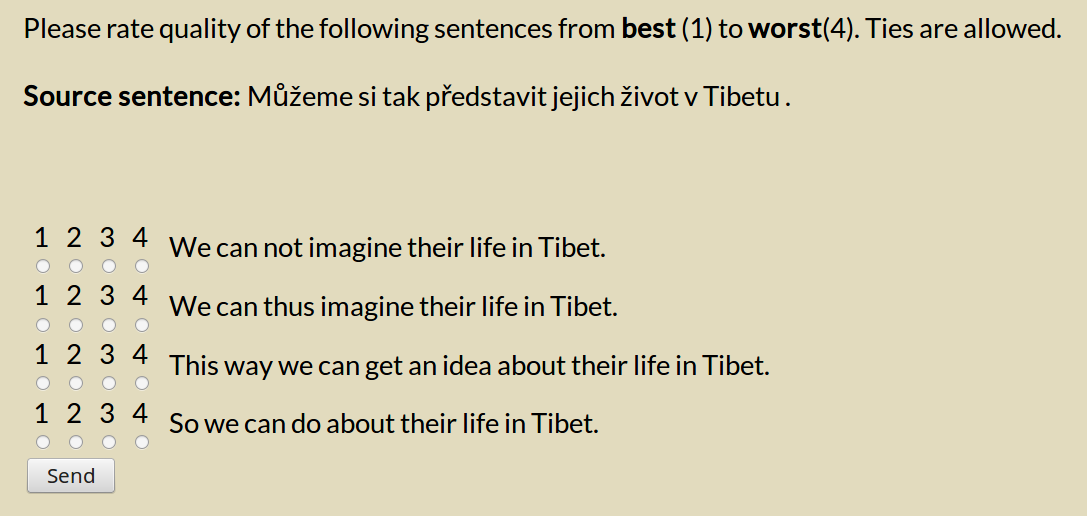
\includegraphics[scale=0.33]{figures/anotovatko.png} 
\caption{Example of the annotation interface for the MT experiment.}
\label{interface}
\end{figure}


We have collected almost 300 comparisons. The inter-annotator agreement 
measured by Krippendorff's alpha \citep{Krippendorff2007}, a~reliability 
coefficient developed to measure the agreement between judges, has achieved
0.58, i.e. a~moderate agreement. The results of replacing the selected verbal 
MWEs by their single verb paraphrases in machine translation are very 
promising: annotators clearly preferred translations of AFTER  (i.e. the 
translations with single verbs) to BEFORE (i.e. with LVCs), in 45\% of cases 
for Moses and in 44\% of cases for Google Translate. The results are consistent
for both translation systems, see \tabref{annotation}.

\begin{table}[tb]
	\centering
	\begin{tabular}{ccc}
	\lsptoprule
		Source & Moses   & GT    \\ \midrule
		BEFORE & 30\%    & 33\%  \\
		AFTER  & 45\%    & 44\%  \\
		TIE    & 25\%    & 23\%  \\
	\lspbottomrule
	\end{tabular}
	\caption{Results of the manual evaluation of the MT experiment. The first 
	column shows the~source of the better ranked sentence in the pairwise 
	comparison within one translation model or whether they tied.}
	\label{annotation}
\end{table}

However, the example in \tabref{example} illustrates that even minimal change in 
a~source sentence can substantially change its translations as both the 
translation models are phrase-based.\footnote{The translations were 
performed on 9th July 2016, i.e. before a massive expansion of neural 
translation systems.} Based on this fact, we can expect that the evaluation of 
the translations was not affected only by differences between translations 
of~LVCs and their respective single verb paraphrases but by overall low quality 
of the translations, which is inevitably reflected in the lower inter-annotator 
agreement, typical of machine translation evaluation \citep{wmt13}. 

\begin{table}[tb]
  \centering
	\scalebox{0.97}{
	\begin{tabular}{llccccc}
		\lsptoprule
		\multirow{6}{*}{Source} & \multirow{3}{*}{BEFORE} & \multicolumn{1}{c}{Fotbalisté}       & Budějovic  & opět  & \multicolumn{1}{c}{\textbf{nedali}} & \textbf{branku} \\
		&                         & \multicolumn{1}{c}{Footballers} & Budějovice & again & \multicolumn{1}{c}{did not give}      & gate   \\
		&                         & \multicolumn{5}{l}{Footballers of Budějovice didn't make a goal again}                               \\ \cline{2-7} 
		& \multirow{3}{*}{AFTER}  & \multicolumn{1}{c}{Fotbalisté}       & Budějovic  & opět  & \multicolumn{2}{l}{\textbf{neskórovali}}               \\
		&                         & \multicolumn{1}{c}{Footballers} & Budějovice & again & \multicolumn{2}{l}{did not score}             \\
		&                         & \multicolumn{5}{l}{Footballers of Budějovice didn't score again}                                     \\ \hline
		\multirow{2}{*}{GT}     & BEFORE                  & \multicolumn{5}{l}{Footballers Budejovice again not given goal}                                           \\ \cline{2-7} 
		& AFTER                   & \multicolumn{5}{l}{Footballers did not score again Budejovice}                                            \\ \hline
		\multirow{2}{*}{Moses}  & BEFORE                  & \multicolumn{5}{l}{Footballers Budějovice again gave the gate}                                            \\ \cline{2-7} 
		& AFTER                   & \multicolumn{5}{l}{Footballers Budějovice score again}                                                    \\ \lspbottomrule
	\end{tabular}
	}
	\caption{An example of translated sentences. The judges unanimously agreed 
	         that the translations of the AFTER source sentence are better than
		     the translations of the BEFORE source sentence. 
		     Both systems exhibited a tendency to translate the LVC \textit{dát branku} 
		     literally word by word, resulting in incorrect translations of the BEFORE 
		     source  sentence.}
	\label{example}
\end{table}



\section{Conclusion}
We have explored the paraphrasability of  Czech light-verb constructions and 
idiomatic verbal constructions. We have shown that their single verb 
paraphrases are automatically obtainable from large monolingual data with 
a~manual verification in a significantly larger scale than from paraphrase 
tables generated from parallel data. Our 
semiautomatic experiment further revealed that although these verbal multiword 
units exhibit different linguistic properties, the possibility to paraphrase 
them is very similar; for about one half of the selected light-verb constructions 
and idiomatic verbal constructions single verb paraphrases have been detected.

The results of our experiment form the lexical stock of a new version of the 
freely available \textit{ParaDi} dictionary. We have demonstrated one of its 
possible applications, namely an experiment with improving machine translation 
quality. However, the dictionary can be used in many other NLP tasks (text 
simplification, information retrieval, etc.). We have used largely language 
independent methods, a similar dictionary can be thus created for other 
languages as well.

\section*{Acknowledgments}
The research reported in this chapter has been supported by the Czech Science 
Foundation GA ČR, grant No. GA15-09979S. This work has been using language 
resources developed and/or stored and/or distributed by the LINDAT-Clarin 
project of the Ministry of Education, Youth and Sports of the Czech Republic, 
project No. LM2015071.

\section*{Abbreviations}
\begin{tabularx}{.49\textwidth}{ll}
\textsc{gt} & Google Translate \\
\textsc{ivc}s & idiomatic verb constructions \\
\end{tabularx}
\begin{tabularx}{.49\textwidth}{ll}
\textsc{lvc}s & light-verb constructions \\
\textsc{mt} & Machine Translation \\
\end{tabularx}


\printbibliography[heading=subbibliography,notkeyword=this]

\end{document}
